\vspace{2ex}
%%%%%%%% Section 4 %%%%%%%%
\section{Computing Optimal \textsf{BaaV} Schemas}
\label{sec-select}

In light of Theorem~\ref{thm-complexity}, any efficient solution
to \baav schema selection is necessarily approximate.
This said, below we develop a practical algorithm 
that given any ``universe'' set $\kb{\A}$ of \bss,
computes the optimal \bds $\kb{\R}$ for $\Q$ that is subsumed by
$\kb{\A}$. That is, it is able to select the optimal $\kb{\R}$
from  $\kb{\A}$ whenever $\kb{\A}$ covers sufficient \bss
including the optimal ones.


Below we present the algorithm assuming a given universe set $\kb{\A}$.
We will study the construction of $\kb{\A}$ in
Section~\ref{sec-cover}.



\begin{myfloat}[t]
\vspace{1.2ex}
\begin{minipage}{0.50\textwidth}
  \removelatexerror
%%%%%%%%%%%%%%%%%%%%% Algorithm: OPTS
{\scriptsize
\setlength{\floatsep}{0cm} % set blank space above the figure
\setlength{\textfloatsep}{-2cm}% set blank space below the figure
\IncMargin{1em}
\vspace{-0.7ex}
\begin{algorithm}[H]
\setstretch{1.1}
%\SetAlgoNoLine
\Indentp{-2ex}
%\DontPrintSemicolon
%\SetAlgoLined
\KwIn{$\Q$ over $\R$, a set
  $\kb{\A}$ of \bss, rank aggregate function $f$.}
\KwOut{\bds $\kb{\R}$ in the normal form for $Q$ with minimum $f(\Q,
  \kb{\R})$ among all normalized \bdss subsumed by $\kb{\A}$.}
\Indentp{1em}
\BlankLine
construct and solve ILP-(I) with
$\kb{\A}$\label{opts-l1}\tcp*[r]{denote its answer by $\kb{\R}_{o}$}
\lIf{$\Q$ is {\em acyclic} \wrt $\kb{\R}_{o}$}{\Return $\kb{\R}_{o}$\label{opts-l2}}
\Else{
  construct and solve ILP-(II) with $\kb{\A}$\label{opts-l4}
  \tcp*[r]{let $\kb{\R}'_{o}$ be its answer}
  \Return $\kb{\R}'_{o}$ \;\label{opts-l5}
}
\caption{Algorithm \opts\label{alg-opts}} 
\end{algorithm}
\DecMargin{1em}
}
%%%%%%%%%%%%%%%%%%%%%
\end{minipage}
\vspace{-2.4ex}
\end{myfloat}


\stitle{Algorithm}.
The main driver of the algorithm, denoted by \opts,
is shown as
Algorithm~\ref{alg-opts}. It takes as input a workload $\Q$ over
database schema $\R$, a set $\kb{\A}$ of \bss and an aggregate rank
function $f(\Q,\ak \kb{\R})$.
It computes the optimal \bds $\kb{\R}$ normalized for $\Q$ from $\kb{\A}$,
\ie for any other \bds $\kb{\R}'\ak \subseteq \ak \kb{\A}$ in the
normal form for $\Q$, $f(\Q,\ak \kb{\R})\ak \leq\ak f(\Q,\ak \kb{\R}')$.
%
Its core idea is to use integer linear programming (ILP) to
express the normal form conditions and ranking criteria of \bdss
for $\Q$, so that computing the optimal normalized \bds in $\kb{\A}$
reduces to solving an ILP program. This allows us to 
capitalize on the latest advances of ILP, \eg algorithms
(cf.~\cite{ILPbook}) and commercial ILP
solvers~\cite{cplex,gurobi,XpressMP}. We use
Gurobi~\cite{gurobi} and IBM CPLEX \cite{cplex}, which can solve,
\eg ILP with 23,000 decision variables and 4,000  constraints
in less than a minute~\cite{ILPstat}, which have far more
variables and constraints than those in our setting.\looseness=-1



The reduction
is challenging since both (a) the normal form and (b) the
scan-free evaluability of \bdss for $\Q$ are semantically defined
and are nontrivial to encode as  an ILP.
% Indeed, (a) is already \NP-hard for generic \SPC queries and
% cannot be exactly captured by linear functions, \eg ILP.

\vspace{1ex}
Despite these, algorithm \opts guarantees the following.

\vspace{-0.3ex}
\begin{theorem}\label{thm-opts}
Algorithm \opts guarantees to compute $\kb{\R}$ from $\kb{\A}$
for $\Q$ such that
(1) $\kb{\R}$ is always in the normal form for $\Q$; and
(2) if $\Q$ consists of K-FK join \SPC queries only, then
\bi
\item[(a)] $\kb{\R}$ is optimal among all \bdss from $\kb{\A}$
  if $\Q$ is {\em acyclic}; 
\item[(b)] $\kb{\R}$ is \ssf-optimal when $\Q$ is cyclic. 
\ei
\vspace{-3.5ex}
\end{theorem}

Here a \bds $\kb{\R}$ normalized for $\Q$ is {\em \ssf-optimal}
({\em strongly scan-free optimal}) \wrt $\kb{\A}$ if $f(\Q, \kb{\R})$
highlights strongly scan-free queries, \ie $\kb{\R}$ is optimal
among all normalized \bdss when $f(\Q, \kb{\R})$ revises
  criterion (1) such that $\usf(Q,\ak \kb{\R}) \ak = \ak 0$ if
  and only if
  (iff) $Q$ is not strongly scan-free over $\kb{\R}$
\warn{(recall Section~\ref{sec-schema} for strongly scan-free evaluability).}
An \SPC
query $Q$ is {\em a key-foreign key (K-FK) join query} if all joins in
$Q$ are K-FK joins.
The {\em acyclicity} of $\Q$ concerns dependencies
in a schema graph, which will be elaborated later on.\looseness=-1

\vspace{0.6ex}
Theorem~\ref{thm-opts} tells us that the \baav schema
$\kb{\R}$ computed by
algorithm \opts is able to answer all \SQL queries posed
on conventional database schema $\R$. Moreover, for 
K-FK join \SPC queries, $\kb{\R}$ guarantees to avoid
costly scans.

\vspace{0.6ex}
We give a constructive proof for Theorem~\ref{thm-opts}
by presenting algorithm \opts. \opts
computes $\kb{\R}$ via two ILP programs,
referred to as ILP-(I) and ILP-(II).
It constructs and solves ILP-(I) (line~\ref{opts-l1}).
Based on its answers \opts decides whether $\Q$ is acyclic,
and returns the \bds encoded in the solution to ILP-(I) if so
(line~\ref{opts-l2}); the \bds is the optimal normalized \bds from
$\kb{\A}$ for K-FK join \SPC queries
(Theorem~\ref{thm-opts}(a)). 
If $\Q$ is cyclic, it then constructs and
solves ILP-(II); it returns the \bds encoded in its solution
(lines~\ref{opts-l4}-\ref{opts-l5}), which
is the \ssf-optimal
normalized \bds from $\kb{\A}$ for K-FK join \SPC queries
(Theorem~\ref{thm-opts}(b)).
\warn{To simplify the presentation of the two ILP programs, we assume
that $\Q$ consists of \SPC queries. For generic \RA (\SQL)
queries, \opts represents them with their max-\SPC sub-queries
in $\Q$ beforehand.}


\vspace{0.8ex}
Below we present the two ILP programs and the identification
of acyclic queries. We then give a proof
of Theorem~\ref{thm-opts}.


\stitle{(1) ILP-(I)}. 
ILP-(I) uses the following 0/1-variables. 
(a)~For each query $Q\in \Q$ , we use $z_{Q}$ to indicate whether
$z_{Q}$ is scan-free over $\kb{\R}$ or not:
$z_{Q} = 1$ iff we pick \bss for $\kb{\R}$ over which $\Q$ is scan-free.
(b)~For each query $Q\in \Q$ and attribute $A$ in $Q$, 
$x_{A}^{Q}$ indicates whether $A$ is ``fetchable'' (see below)
from constants
in $Q$ over $\kb{\R}$. 
(c)~For each \bs $\kb{R}$, $y_{\kb{R}}$ indicates
whether $\kb{R}$ is picked for $\kb{\R}$, and $y^{Q}_{\kb{R}}$ 
indicates whether $\kb{R}$ is picked in order to make $Q$ scan-free
for each $Q\in \Q$.
%\looseness = -1

\vspace{0.36ex}
We also use the following notations. For a \bs $\kb{R}$,
denote by $X_{\kb{R}}$ and $Y_{\kb{R}}$ the attributes such that
$\kb{R}\ak =\ak  \bschema{X_{\kb{R}}}{Y_{\kb{R}}}$.
We use $A$ to denote an attribute, and $R$ to denote a
relation schema in $\R$.
Denote by $\A_{R}$ the set of \bss $\kb{R} \ak = \ak
\bschema{X}{Y}$ with $Y$ from relation schema $R$. For an
attribute $A$ of $\R$, denote by $\RHS(A)$ the set of all \bss
$\kb{R}$ in $\kb{\A}$ such that $A\in Y_{\kb{R}}$.
%
For each parametric query $Q$ in $\Q$, denote by $P_{Q}$ the set
of parameters of $Q$; denote by $Y_{Q}$ all the other
attributes appearing %appeared
in the predicates of $Q$ that
are in the form of relational
algebra (\ie $Y_{Q}$ includes attributes that appear %appeared
in joins or project predicates of $Q$). 
\looseness = -1

\vspace{0.36ex}
For each $Q$ in $\Q$ and each relation atom $R$ in $Q$, denote by
$W_{R}$ the \qcs~\cite{blinkdb} of $Q$ on $R$ (\ie attributes of
$R$ that are also in $P_{Q}Y_{Q}$ of $Q$); denote by $\Wc_{\Q}$
the set of all \qcs of queries in $\Q$. For each \qcs $W$ in
$\Wc_{\Q}$, denote by $\kb{\R}_{W}$ the set of \bss $\kb{R}\ak
=\ak \bschema{X}{Y}$ in $\kb{\A}$ that {\em support} $W$, \ie
$W\ak\subseteq\ak XY$. 

% As will be shown shortly, if all \qcs of a query $Q$ are
% supported by a set $S$ of \bss, then $S$ is a cache database
% schema that is in normal form for $Q$.

\vspace{0.6ex}
Then program ILP-(I) is constructed as follows.

\vspace{-1ex}
\begin{tcolorbox}[
  blanker,
  breakable,
  ]
  \begin{alignat}{2}
\hspace{-2.6cm}\text{minimize:
} & c_{1}f_{1}+c_{2}f_{2}+c_{3}f_{3} & \hfill
  \end{alignat}
  
  \vspace{-3.3ex}
  
  \begin{alignat}{2}
   \hspace*{-0.15cm}\text{subject to: }&  x_{A}^{Q} = 1 & \forall
    A\in P_{Q}, \forall Q \\[0.8ex] 
    & z_{Q}\leq x_{A}^{Q} & \forall A \in Y_{Q},\forall Q \\[0.8ex]
    & x_{A}^{Q} \leq\textstyle \sum_{\kb{R}\in \RHS(A)}\!y_{\kb{R}}^{Q} &~\forall
    A\not\in P_{Q}, \forall Q \\[0.8ex]
    & y_{\kb{R}}^{Q} \leq x_{A}^{Q} & \forall \kb{R}\in \kb{\A}, \forall A\in X_{\kb{R}}, \forall
    Q\\[0.8ex]
    & \textstyle \sum_{\kb{R}\in \A_{R}} y_{\kb{R}}^{Q} \leq 1 & 
    \forall R\in \R, \forall Q \\[0.8ex]
    & y_{\kb{R}}^{Q} \leq y_{\kb{R}} & \forall Q, \forall \kb{R} \\[0.8ex]
    & \textstyle\sum_{\kb{R}\in \kb{R}_{W}} y_{\kb{R}} \geq 1 & \forall W\in \Wc_{\Q} \\[0.8ex]
    %& x_{A}^{Q} \in \{0, 1\} & \forall A\text{ in }\R, \forall
    %Q\\[0.8ex]
    & z_{Q}, x_{A}^{Q} \in \{0, 1\} & \forall
    A\text{ in }\R, \forall Q\\[0.8ex]
    & y_{\kb{R}}, y_{\kb{R}}^{Q} \in \{0, 1\} & \forall Q, \forall
    \kb{R} 
  \end{alignat}
  \end{tcolorbox}

\vspace{-0.7ex}

\sstab
where $c_{i} (i\in[1, 3])$  in (1) are coefficients adjustable
by the users when specifying the
optimization objective,  $\sum_{i=1}^{3}c_{i} = 1$ (recall
from Section~\ref{sec-rank}), and $f_{i}(i\in [1, 3])$ are:
  $f_{1} = \textstyle\sum_{Q\in \Q} (1-z_{Q})$,
  $f_{2} = \textstyle\sum_{\kb{R}\in \kb{\A}} y_{\kb{R}}*|Y_{\kb{R}}|$,
  and
  $f_{3} = \textstyle\sum_{\kb{R}\in \kb{\A}} y_{\kb{R}}*|\kb{R}|$.


 \vspace{0.6ex}
Below we give intuition behind the ILP program.
Equation (2) above indicates that all
attributes in $P_{Q}$ are ``known'' for $Q$ already; to make
$Q$ scan-free, we need to fetch $Y_{Q}$-values (partial tuples) associated
with such known $P_{Q}$-values via selected \bss for
$Q$, which are indicated by $y_{\kb{R}}^{Q}$.
Inequation (3) ensures that when a query $Q$ is made scan-free (\ie
$z_{Q} = 1$), all attributes in $Y_{Q}$ should be also be
{\em fetchable}, where an attribute is fetchable in $Q$
when it can be retrieved from $P_{Q}$ via $\get(k)$ over picked
\bss without scans.


\vspace{0.6ex}
Inequation (4) enforces that when an attribute $A$ is fetchable in
$Q$ (\ie $X_{A}^{Q} = 1$), $A$ must be either in $P_{Q}$ or
in $Y_{\kb{R}}$ of some \bs $\kb{R}$ ($\kb{R} \in \RHS(A))$
that has been picked for $Q$, \ie $y_{\kb{R}}^{Q} = 1$.

Inequation (5) further enforces that attribute $A$ in $X_{\kb{R}}$
of $\kb{R}$ in $Q$ must be fetchable if $\kb{R}$ is picked for $Q$.

\vspace{0.6ex}
Inequation (6) is to ensure that for each relation $R$ in $\R$,
only one \bs $\kb{R} \ak =\ak \bschema{X}{Y}$ with $Y$ from $R$ is used
to make $Q$ scan-free; this is to ensure that when all $Y_{Q}$ attributes
can be fetched from $P_{Q}$-values, they are warranted to come from
the same tuples in the database instance $\D$ of $\R$, \ie their
combinations do not generate ``false'' $Y_{Q}$-values that are
not in $\D$.
\looseness = -1

\vspace{0.8ex}
When taken together,
constraints (2)-(6) ensure that if $z_{Q}\ak
=\ak 1$, \ie~if $Q$ is scan-free over \bss $\kb{R}$ picked for $Q$
($y_{\kb{R}}^{Q}\ak =\ak 1$), for each $A$ in $Y_{Q}$,
there must exist a sequence of \get operations that can retrieve
$A$ over the picked \bss starting from parameters $P_{Q}$ of $Q$
(assuming that the picked \bss are ``acyclic'', which we will
elaborate shortly).

\vspace{0.6ex}
Inequation (7) ensures that when $Q$ picks a \bs $\kb{R}$
($y_{\kb{R}}^{Q} = 1$), $\kb{R}$ is included in \bds $\kb{\R}$
($y_{\kb{R}} = 1$).
%
Inequation (8) is to guarantee that any feasible solution to the
ILP program must yield a \bds that is in the normal form for all
queries in $\Q$: for each \qcs $W$ of $\Q$, $W$ is supported by
at least a \bs picked in $\kb{\R}$.\looseness=-1

\vspace{0.6ex}
Equations (9)-(10) claim that all variables are either 0 or 1.


\vspace{1.6ex}
Algorithm \opts constructs and solves ILP-(I), 
by using existing ILL solvers, \eg Gurobi~\cite{gurobi} or
IBM CPLEX~\cite{cplex}.
%
It then interprets \bdss from solutions to the ILP
program: for any feasible solution (\ie 0/1 assignment to the
variables), it construct \bds $\kb{\R}$ that consists of \bss
$\kb{R}$ in $\kb{\A}$ with $y_{\kb{R}}  = 1$ in the feasible
solution. We refer to such $\kb{\R}$ {\em the \bds encoded by the
solution to ILP program}. \opts returns the \bds
$\kb{\R}_{o}$ encoded by the optimal solution to ILP-(I) only
when $\Q$ is acyclic \wrt $\kb{\R}_{o}$ (line~\ref{opts-l2}), which we elaborate below. 


\begin{example}\label{exa-ILP-I}
Continuing with Example~\ref{exa-measures},
let the universe set $\kb{\A}$ be $\kb{\R}_{2}$.
By constructing and solving the ILP-(I) with $\kb{\R}_{2}$ and $\Q$,
one can verify that the optimal assignment to ILP-(I) has
$z_{Q_{1}} = 1$, $y_{\kb{\at{T}}_{1}} = y_{\kb{\at{C}}_{1}} =
y_{\kb{\at{B}}_{1}} = 1$ and $y_{\kb{R}} = 0$ for all other
$\kb{R}$ in $\kb{\R}_{2}$, with the objective of ILP-(I) scored $0.1$, which
exactly matches $f_{0}(\Q, \kb{\R}_{1})$ calculated in Example~\ref{exa-measures}.
Note that the encoded \bds by this assignment is also exactly
$\kb{\R}_{1}$. This shows that ILP-(I) correctly computes the
score of $\kb{\R}_{1}$ for $\Q$ and identifies it as the optimal
\bds within $\kb{\R}_{2}$ for $\Q$ under $f_{0}$. 
\end{example}
\looseness = -1


\stitle{(2) Acyclicity checking}. Below we
first exemplify the notion
of acyclicity of a query $Q$ \wrt the \bds $\kb{\R}_{o}$ encoded
in the optimal solution to ILP-(I). Let $\kb{\R}_{Q}$ be the set
of \bss $\kb{R}$ in $\kb{\R}_{o}$ with $y_{\kb{R}}^{Q} = 1$ in
the solution to ILP-(I).


\begin{example}\label{exa-acyclicity}
Continuing with Example~\ref{exa-ILP-I}, let
the universe set $\kb{\A}$   be $\kb{\R}_{3}$.
By constructing and solving ILP-(I) with $\kb{\R}_{3}$ and $\Q$,
one can find the following.
(1) The optimal assignment to ILP-(I) has
$z_{Q_{1}} = 1$, $y_{\kb{\at{TC}}_{1}} = y_{\kb{\at{B}}_{1}} =
y_{\kb{\at{B}}_{2}} = 1$ and $y_{\kb{\at{C}}_{1}} = 0$; its
objective score is $0.98*0\ak +\ak 0.01*3\ak +\ak 0.01*8\ak =\ak
0.11$.
(2) The \bds encoded by this assignment, denoted by $\kb{R}_{4}$,
consists of $\kb{\at{TC}}_{1}$, $\kb{\at{B}}_{1}$ and
$\kb{\at{B}}_{2}$.
(3) However, $f_{0}(\Q, \kb{\R}_{4}) = 1.09$. Indeed, in contrast to
what $z_{Q_{1}}= 1$ indicates, $Q_{1}$ is not scan-free over
$\kb{\R}_{4}$ since one cannot fetch \at{city} values from
\at{date} and \at{payee} over $\kb{\R}_{4}$ without scanning
$\kb{\at{TC}}_{1}$; that is, $\usf(\Q, \kb{\R}_{4}) = 1$ and
thus $f_{0}(\Q, \kb{\R}_{4})$ is inconsistent with the
objective of ILP-(I).

\vspace{0.6ex}
The reason that ILP-(I) cannot capture $f(\Q, \kb{\R}_{4})$ is
because $\kb{\R}_{4}$ is {\em cyclic} for $Q$ as observed by the optimal
assignment to ILP-(I). When minimizing its objective, ILP-(I)
finds that $z_{Q}\ak =\ak 1$ meets constraints (2)-(6) of ILP-(I)
when $y_{\kb{\at{B}}_{1}}\ak =\ak y_{\kb{\at{B}}_{2}}\ak =\ak 1$, while
\at{city} cannot be fetched with $\kb{\at{B}}_{1}$ and
$\kb{\at{B}}_{2}$ from \at{date} and \at{payee}, since
$\kb{\at{B}}_{1}$ and $\kb{\at{B}}_{2}$ form a {\em cycle} with
their attributes: $\kb{\at{B}}_{1}$ fetches \at{city} for $Q_{1}$
if \at{bid} attributes can be fetched, while \at{bid} can be
fetched via $\kb{\at{B}}_{2}$ when \at{city} is known. Therefore,
$z_{Q}$ can be assigned with 1 when both $\kb{\at{B}}_{1}$ and
$\kb{\at{B}}_{2}$ are picked by $y_{\kb{\at{B}}_{1}}^{Q}$ and
$y_{\kb{\at{B}}_{2}}^{Q}$ for $Q$ in ILP-(I). This demonstrates that ILP-(I)
cannot capture the scan-free evaluability of
$\kb{\R}_{4}$ for $Q_{1}$ when it is cyclic.
\end{example}
\looseness = -1

As shown in Example~\ref{exa-acyclicity}, if $\kb{\R}_{Q}$ is
``cyclic'', attribute $A$ in $Y_{Q}$ of $Q$ cannot always be
fetched from parameters $P_{Q}$ of $Q$ even when $x_{A}^{Q} = 1$,
where $\kb{\R}_{Q}$ consists of all \bss $\kb{R}$ in $\kb{\R}_{o}$
with $y_{\kb{R}}^{Q} = 1$ in the solution to ILP-(I) (\ie
$\kb{\R}_{4}$ for $Q_{1}$ with $\kb{\A} = \kb{\R}_{2}$).
In other words, ILP-(I) alone cannot capture the scan-free
evaluability of $\kb{\R}_{Q}$ and hence it may not be optimal anymore. 
\looseness = -1

%\warn{Do you mean ``cyclic'' instead above? Not very logical}

We next formalize the acyclicity of \bds $\kb{\R}_{Q}$ for $Q$.
% As will be shown shortly, if $\A_{Q}$ in $\A$ identified
% by the ILP program is acyclic for each $Q$ in $\Q$, \opts safely
% returns $\A$ as the optimal \cds for $\Q$.
This is based on a graph representation of $\kb{\R}_{Q}$, referred to
as the {\em schema graph} of $\kb{\R}_{Q}$ and denoted by
$G_{\kb{\R}_{Q}}$.


\eetitle{Schema graph}. More specifically, $G_{\kb{\R}_{Q}}$ is a
directed graph constructed from $\kb{\R}_{Q}$ as follows: each \bs
$\kb{R} = (X\ra Y)$ is represented in $G_{\kb{\R}_{Q}}$ as $|X|+|Y|+1$
nodes and $|X|+|Y|$ edges:
\looseness = -1
\mbi
\item each attribute $A$ in $X$ and $Y$ is a node $u_{A}$ in $G_{\kb{\R}_{Q}}$;
\item $G_{\kb{\R}_{Q}}$ additionally encodes set $Y$ as a node $u_{Y}$;
\item $(u_{A}, u_{Y})$ is an edge in $G_{\kb{\R}_{Q}}$ for each $A\in X$; and
\item $(u_{Y}, u_{A})$ is an edge in $G_{\kb{\R}_{Q}}$ for each attribute $A\in Y$.
\mei 

\begin{figure}
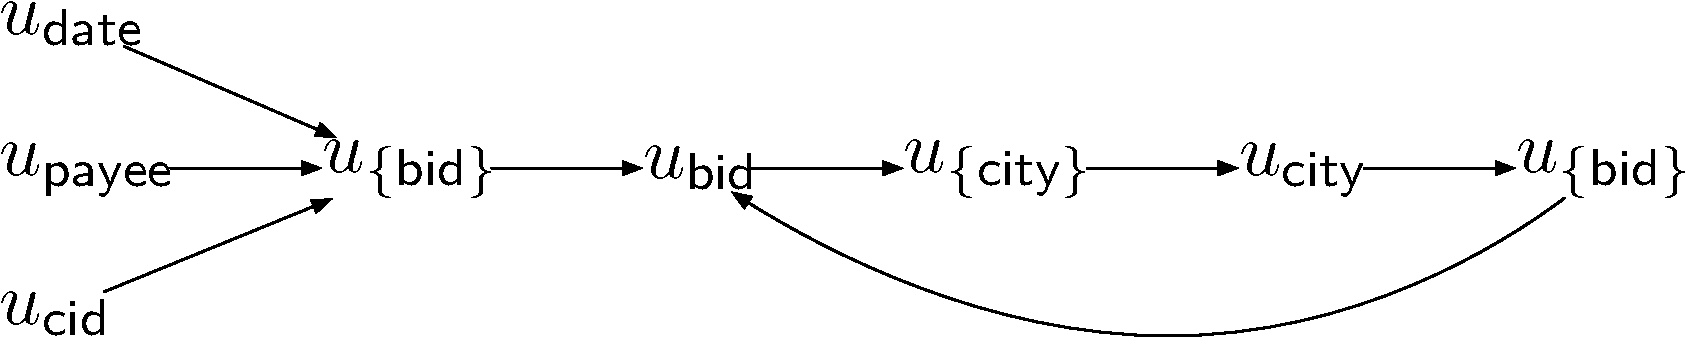
\includegraphics[width=1\columnwidth]{fig/schemagraph.pdf}
\caption{The schema graph of $\kb{\R}_{Q_{1}}$ (\ie
  $\kb{\R}_{4}$) \label{fig-schemagraph}}
\vspace{-2ex}
\end{figure}

\begin{example}\label{exa-schemagraph}
The schema graph of $\kb{\R}_{Q_{1}}$ (\ie $\kb{\R}_{4}$) for
$Q_{1}$ with $\kb{\A} = \kb{\R}_{2}$ is depicted in
Fig.~\ref{fig-schemagraph}. The graph is cyclic.
\end{example}


\eetitle{Acyclicity}.
We say that $\kb{\R}_{Q}$ is {\em acyclic \wrt $\kb{\R}_{o}$} if schema
graph $G_{\kb{\R}_{Q}}$ is acyclic; otherwise $\kb{\R}_{Q}$ is
{\em cyclic}. Query $Q$ is {\em acyclic} \wrt $\kb{\R}_{o}$ if
$\kb{\R}_{Q}$ is acyclic \wrt $\kb{\R}_{o}$. A workload $\Q$ is
{\em acyclic} \wrt $\kb{\R}_{o}$ if each query in $\Q$ is acyclic \wrt
$\kb{\R}_{o}$.


\vspace{0.8ex}
Algorithm \opts checks whether $\Q$ is acyclic \wrt the optimal
solution $\kb{\R}_{o}$ to ILP-(I), and returns $\kb{\R}_{o}$ 
if $\Q$ is acyclic (line~\ref{opts-l2}). However, if $\Q$ is
cyclic, $\kb{\R}_{o}$ may not be optimal since the ILP-(I) cannot
capture the scan-free evaluability of $\kb{\R}_{o}$;
for such cases, \opts further triggers ILP-(II) below.


\vspace{0.36ex}

\stitle{(3) ILP-(II)}.
For cyclic queries,
ILP-(II) computes %only
\ssf-optimal normalized \bds $\kb{\R}_{o}'$ for $\Q$. 
To do so, ILP-(II) %is almost the same as ILP-(I) except that it
extends ILP-(I) with an additional constraint besides the constraints
of ILP-(I):\looseness=-1
\vspace{-0.7ex}
\begin{alignat}{2}                                                       
&  y_{\kb{R}}^{Q} = 0 &~~~~~~~~~~~~\forall \kb{R}, \forall Q, X_{\kb{R}}\not\subseteq P_{Q}
\end{alignat}                                                            

\vspace{-0.7ex}

Intuitively, equation (11) allows ILP-(II) to enforce that when
selecting \bss to make query $Q$ scan-free, for each
\bs $\kb{R} \ak = \ak \bschema{X}{Y}$ it picks for $Q$, $X\subseteq
P_{Q}$, \ie $Q$ can be answered with $\get(k)$ operations where
$k$'s are the parameters of $Q$.
%\looseness = -1


\vspace{0.36ex}
When $\Q$ is cyclic \wrt the \bds $\kb{\R}_{o}$ encoded by the
optimal solution to ILP-(I), algorithm \opts constructs and solves
ILP-(II), and returns the \bds $\kb{\R}_{o}'$ encoded by the
optimal solution to ILP-(II), \ie $\kb{\R}_{o}'$ consists of \bss
$\kb{R}$ in $\kb{\A}$ with $y_{\kb{R}} = 1$. 

\begin{example}\label{exa-ILP-II}
With $\kb{\R}_{3}$, \opts computes an optimal assignment to
ILP-(II) that has $z_{Q} = 0$, %$x_{\at{city}} = 0$,
$y_{\kb{\at{TC}}_{1}} = y_{\kb{\at{B}}_{1}} = 1$ and
$y_{\kb{\at{B}}_{2}} = y_{\kb{\at{C}}_{1}} = 0$. %, which
This encodes a
\bds $\kb{\R}_{5}$ consisting of $\kb{\at{B}}_{1}$ and
$\kb{\at{TC}}_{1}$ for query load $\Q$. Note that the objective of ILP-(II)
with this assignment is 1.06, which is consistent with $f_{0}(\Q,
\kb{\R}_{5})$. 
\end{example}

\vspace{-0.4ex}

\stitle{Analysis}. We next prove Theorem~\ref{thm-opts} with the following lemmas. 



\begin{lemma}\label{lem-ILP-norm}
  For any \SQL $Q$, if for each \qcs $W$ in $\Wc_{Q}$ there
  exists a \bs $\kb{R}$ in $\kb{\R}$ that supports $W$, then
  $\kb{\R}$ is in the normal form for $Q$.
\end{lemma}
\looseness = -1

Lemma~\ref{lem-ILP-norm} is straightforward from the following observations:
(a) a query $Q$ can be answered if all of its \qcs values can be
retrieved; moreover,
(b) if a \qcs $W$ is supported by a \bs $\kb{R}$, then by scanning
$\kb{R}$ one could retrieve all the $W$-values. 

Note that the condition of Lemma~\ref{lem-ILP-norm} is enforced
by inequation (8) for each query $Q$ in $\Q$.
Hence, by Lemma~\ref{lem-ILP-norm}, any feasible solution to ILP-(I)
or ILP-(II) must encode a \bds that is in the normal form for $\Q$.
This verifies Theorem~\ref{thm-opts}(1). 


\vspace{1ex}
For feasible solutions to ILP-(I) and ILP-(II) and the
corresponding \bdss $\kb{\R}$ encoded by them,
we have the following.

\vspace{-0.5ex}
\begin{lemma}\label{lem-ILP}
  For any K-FK join \SPC query $Q$ in $\Q$, 

  \sstab (1) $Q$ is scan-free over some \bds $\kb{\R}$ only if there exists a feasible
  solution to ILP-(I) with $z_{Q} = 1$; 

  \sstab (2) $Q$ is scan-free evaluable over $\kb{\R}$
  if there is a \bds $\kb{\R}$ encoded by a feasible
  solution to ILP-(I) with $z_{Q} = 1$ and $Q$ is acyclic \wrt
  $\kb{\R}$; and

  \sstab (3) $Q$ is strongly scan-free evaluable iff there exist a
  feasible solution to ILP-(II) with $z_{Q} = 1$. 
\end{lemma}

\vspace{-0.7ex}


\begin{proofS}
% All three results can be proved by induction on $(m, n, p)$,
% where $m$ is $\cdd{\Q}$, \ie the number of $z_{Q}$ variables; $n$
% is the number of $x_{A}^{Q}$ variables; $p$ is the number of
% $y_{\kb{R}}$ variables, \ie the number of \bss in $\kb{\R}$.
%In particular, to prove (1), the key observation for the
%induction is the following:
All the three results can be proved by induction. 
%In particular,
To prove (1), observe that when $Q$ is scan-free
over some \bds $\kb{\R}$, by definition there must exist a chain
(\ie plan)
of \get operations that can retrieve $A$ from parameters of $Q$
for each $A\in Y_{Q}$. One can verify by induction on the length
of the chain that each chain encodes a partial assignment to the
0/1-variables that satisfies the constraints of ILP-(I) and leads to
$x_{A}^{Q} = 1$ for each $A\in Y_{Q}$. By inequation (3), such
partial assignments, together with $z_{Q} = 1$, form a feasible
solution (\ie assignment) that satisfies all the constraints
in ILP-(I).
%
One can verify
(2) along the same lines. By induction on $(m, n)$,
where $m$ is the number of $x_{A}^{Q}$ variables and $n$ is the
number of $y_{\kb{R}}$ variables (\ie the number of \bss in
$\kb{\A}$) in ILP-(I), one can construct a scan-free query plan
over $\kb{\R}$ from the assignment of any feasible solution. The
key step is that when $Q$ is acyclic \wrt $\kb{\R}$, for each
$x_{A}^{Q} = 1$ for some $A\in Y_{Q}$, one can always trace back
to $x_{A'}^{Q} = 1$ for some parameters $A\in P_{Q}$, such that
the trace encodes a fetching plan for $A$ from $A'$.
For (3), the if (resp.~only if) direction follows from the proof
of (2) (resp.~(1)), and is simpler. 
\end{proofS}
\looseness = -1

Lemma~\ref{lem-ILP} considers \SPC queries with K-FK joins 
since all the analysis is based on that $Q$ is
(resp.~strongly) scan-free iff $\bschema{P_{Q}}{Y_{Q}}$ is
implied by $\kb{\R}$, \ie there exists a (resp.~strongly) scan-free
plan over $\kb{\R}$ that fetches attributes in $Y_{Q}$ over
$\kb{\R}$, starting from $P_{Q}$. Such a prerequisite holds for
\SPC queries in which joins are all K-FK joins.
\looseness = -1

Putting these together, we are now ready to prove
  Theorem~\ref{thm-opts}.

\vspace{0.8ex}
\noindent
    {\bf Proof of Theorem~\ref{thm-opts}}. As remarked earlier,
    Theorem~\ref{thm-opts}(1) follows from Lemma~\ref{lem-ILP-norm}.
To show  Theorem~\ref{thm-opts}(2a), observe that
by Lemma~\ref{lem-ILP}(1), feasible solutions to ILP-(1) can
cover all \bdss over which $Q$ is scan-free. This ensures that
the \bds $\kb{\R}_{o}$ encoded by the optimal solution to ILP-(1)
must have the minimum ranking score.
%, although its ``true''
%score of $\usf(\Q,\ak \kb{\R}_{o})$ (\ie~measure (1)) may be worse.
Lemma~\ref{lem-ILP}(2) ensures that if $\Q$ is
acyclic \wrt $\kb{\R}_{o}$ then its score of $\usf(\Q,\ak
\kb{\R}_{o})$ is measured correctly in the optimal solution to
ILP-(I); hence $\kb{\R}_{o}$ is the optimal \bds for $\Q$. This
verifies Theorem~\ref{thm-opts}(2a).
%\looseness = -1

\vspace{0.6ex}
For Theorem~\ref{thm-opts}(2b),
Lemma~\ref{lem-ILP}(3) tells us that feasible solutions to
ILP-(II) can encode all \bdss over which $\Q$ is strongly
scan-free, \ie the \bds $\kb{\R}_{o}'$ encoded by the optimal
solution to ILP-(II) is measured correctly
%\wrt all the measures via the ILP program
when the strong scan-free evaluability is
adopted. Hence, $\kb{\R}_{o}'$ must always be \ssf-optimal for
$\Q$. This verifies Theorem~\ref{thm-opts}(2b). \eop
\looseness = -1


\eetitle{Complexity}. Algorithm \opts is in
$O(\cd{\kb{\A}}\cd{\Q} + T_{\at{ILP}} )$-time, where
$\cd{\kb{\A}}$ and $\cd{\Q}$ are the total number of attributes
in $\kb{\A}$ and $\Q$ (in the predicates of its algebra form),
respectively, and $T_{\at{ILP}}$ is the time for solving the ILP programs. 
Indeed, %note the following:
(a) it takes $O(\cd{\Q}\cd{\kb{\A}})$ time to construct ILP-(I) and
ILP-(II) with $\kb{\A}$.
(b) There are $\cdd{\Q} + \cdd{\Q}\cd{\A} + \cdd{\kb{\R}} + \cdd{\kb{\A}}\cdd{\Q}$ 0/1
variables in both ILP programs.
(c) ILP-(II) and ILP-(I) have at most
$3\cdd{\Q}\cdd{\kb{\A}} + 5\cdd{\Q}\cd{\R} + \cd{\Q} +
\cdd{\Q} + \cdd{\kb{\A}} + \cd{\kb{\A}}\cdd{\Q}$ linear
constraints, where $\cd{\R}$ is the total number of attributes in
$\R$, $\cdd{\Q}$ is the number of queries in $\Q$ and
$\cdd{\kb{\A}}$ is the number of \bss in $\kb{\A}$.\looseness=-1 



\stitle{Remark}. Algorithm \opts is generic and can be easily
adapted to serve various scenarios. Below are a few examples.

\sstab (1) One can treat some of the measures of \opts
as constraints. For instance, if users
want to find optimal normalized \bds with size bounded by a
storage budget $B$, then they can simply move $f_{3}$ from the
objective (1) of ILP-(I) and ILP-(II) to a constraint 
$f_{3}\leq B$.

\sstab (2) One can even specify certain queries $Q$ and request
to make them scan-free over the returned \bds $\kb{\R}$. This is
easily done by adding additional constraints $z_{Q} = 1$
for the pick queries.

\sstab (3) By controlling $c_{i}$ in the rank aggregate function
$f(\Q, \kb{\R})$, one can prioritize certain
measures. For example, if users care more about the
  performance of query answering than
  %while downplaying
the maintenance cost, \eg when querying static historical data,
they could assign $c_{1}$ a
  large coefficient, %followed by a moderate $c_{2}$,
  and set $c_{4}$
to 0.

\eat{%EAT
  \section{Selecting top-$k$ Optimal Schemas}
\label{sec-select}

In light of Theorem~\ref{thm-complexity}, any efficient solution
to \bdsd is necessarily approximate.
Nonetheless, below we develop a practical algorithm for \bdsd
that can compute, given any universe set $\kb{\A}$ of \bss,
the optimal \bds $\kb{\R}$ for $\Q$ that is subsumed by
$\kb{\A}$. Hence, whenever $\kb{\A}$ subsumes the optimal
$\kb{\R}$ for $\Q$, the algorithm can identify and return it from
$\kb{\A}$.

Below we present the algorithm with a given universe set $\kb{\A}$.
We will study the construction of $\kb{\A}$ in
Section~\ref{sec-cover}.



\begin{myfloat}[t]
\vspace{1.2ex}
\begin{minipage}{0.50\textwidth}
  \removelatexerror
%%%%%%%%%%%%%%%%%%%%% Algorithm: OPTS
{\scriptsize
\setlength{\floatsep}{0cm} % set blank space above the figure
\setlength{\textfloatsep}{-2cm}% set blank space below the figure
\IncMargin{1em}
\vspace{-0.7ex}
\begin{algorithm}[H]
\setstretch{1.1}
%\SetAlgoNoLine
\Indentp{-2ex}
%\DontPrintSemicolon
%\SetAlgoLined
\KwIn{$\Q$ over $\R$, set $\kb{\A}$ of \bss, rank aggregate function $f$.}
\KwOut{\bds $\kb{\R}$ in normal form for $Q$ with minimum $f(\Q,
  \kb{\R})$ among all normalized \bdss subsumed by $\kb{\A}$.}
\Indentp{1em}
\BlankLine
construct and solve ILP-(I) with
$\kb{\A}$\label{opts-l1}\tcp*[r]{denote its answer by $\kb{\R}_{o}$}
\lIf{$\Q$ is {\em acyclic} \wrt $\kb{\R}_{o}$}{\Return $\kb{\R}_{o}$\label{opts-l2}}
\Else{
  construct and solve ILP-(II) with $\kb{\A}$\label{opts-l4}
  \tcp*[r]{let $\kb{\R}'_{o}$ be its answer}
  \Return $\kb{\R}'_{o}$ \;\label{opts-l5}
}
\caption{Algorithm \opts\label{alg-opts}} 
\end{algorithm}
\DecMargin{1em}
}
%%%%%%%%%%%%%%%%%%%%%
\end{minipage}
\vspace{-2.4ex}
\end{myfloat}


The algorithm, denoted by \opts and shown as
Algorithm~\ref{alg-opts}, takes as input a workload $\Q$ over
database schema $\R$, a set $\kb{\A}$ of \bss and an aggregate rank
function $f(\Q,\ak \kb{\R})$.
It computes the optimal \bds $\kb{\R}$ normalized for $\Q$ from $\kb{\A}$,
\ie for any other \bds $\kb{\R}'\ak \subseteq \ak \kb{\A}$ that is in
normal form for $\Q$, $f(\Q,\ak \kb{\R})\ak \leq\ak f(\Q,\ak \kb{\R}')$.
%
Its core idea is to use integer linear programming (ILP) to
express the normal form conditions and ranking measures of \bdss
for $\Q$, so that computing the optimal normalized \bds in
$\kb{\A}$ reduces to solving an ILP program. This allows us to
employ the latest advances of ILP, \eg algorithms
(cf.~\cite{ILPbook}) and commercial ILP
solvers~\cite{cplex,gurobi,XpressMP}.


This is challenging since both (a) the normal form and (b) the
scan-free evaluability of \bdss for $\Q$ are semantically defined
and may not be able to directly encoded by an ILP.
% Indeed, (a) is already \NP-hard for generic \SPC queries and
% cannot be exactly captured by linear functions, \eg ILP.

\vspace{1ex}
Nonetheless, \opts guarantees the following. We say that
a \bds $\kb{\R}$ normalized for $\Q$ is {\em \ssf-optimal}
({\em strongly scan-free optimal}) \wrt $\kb{\A}$ if $f(\Q, \kb{\R})$
concerns strongly scan-free queries, \ie $\kb{\R}$ is optimal
among all normalized \bdss when $f(\Q, \kb{\R})$ uses strongly
scan-free to for measure (1): $\sf(Q,\ak \kb{\R}) \ak = \ak 1$
iff $Q$ is strongly scan-free over $\kb{\R}$. We say an \SPC
query $Q$ is a key-foreign key (K-FK) join query if all joins in
$Q$ are K-FK joins.
\looseness = -1

\vspace{-0.3ex}
\begin{theorem}\label{thm-opts}
Algorithm \opts guarantees to compute $\kb{\R}$ from $\kb{\A}$
for $\Q$ such that
(1) $\kb{\R}$ is always in normal form for $\Q$; and
(2) if $\Q$ consists of K-FK join \SPC queries only, then
\bi
\item[(a)] $\kb{\R}$ is optimal among all \bdss from $\kb{\A}$
  if $\Q$ is {\em acyclic}; 
\item[(b)] $\kb{\R}$ is \ssf-optimal when $\Q$ is cyclic. 
\ei
\vspace{-3.5ex}
\end{theorem}

We will elaborate the {\em acyclicity} of $\Q$ shortly.

Algorithm \opts computes $\kb{\R}$ via two ILP programs,
referred to as ILP-(I) and ILP-(II).
It constructs and solves ILP-(I) (line~\ref{opts-l1}),
via whose answer it decides whether $\Q$ is acyclic and
returns the \bds encoded in the solution to ILP-(I) if so
(line~\ref{opts-l2}), which is the optimal normalized \bds from
$\kb{\A}$ for \SPC with K-FK joins only
(Theorem~\ref{thm-opts}(a)). 
If it identifies that $\Q$ is cyclic, it then constructs and
solves ILP-(II) and returns the \bds encoded in its solution
(lines~\ref{opts-l4}-\ref{opts-l5}), which is the \ssf-optimal
normalized \bds from $\kb{\A}$ for \SPC with K-FK joins
(Theorem~\ref{thm-opts}(b)).
\looseness = -1


\vspace{0.8ex}
Below we present the two ILP programs and show how \opts
identifies acyclic queries $\Q$. 


\stitle{(a) ILP-(I)}. 
ILP-(I) uses the following 0/1-variables: 
(a)~For each query $Q\in \Q$ , we use $z_{Q}$ to indicate whether
$z_{Q}$ is scan-free over $\kb{\R}$ or not:
$z_{Q} = 1$ indicates we pick \bss for $\kb{\R}$ over which $\Q$ is scan-free.
(b)~For each query $Q\in \Q$ and attribute $A$ in $Q$, we use
$x_{A}^{Q}$ to indicate whether $A$ is fetchable from constants
in $Q$ over $\kb{\R}$. 
(c)~For each \bs $\kb{R}$, we use $y_{\kb{R}}$ to indicate
whether $\kb{R}$ is picked for $\kb{\R}$, and use $y^{Q}_{\kb{R}}$ to
indicate whether $\kb{R}$ is picked in order to make $Q$ scan-free
for each $Q\in \Q$.
\looseness = -1

\vspace{0.4ex}
We also use the following notations. For a \bs $\kb{R}$,
denote by $X_{\kb{R}}$ and $Y_{\kb{R}}$ the attributes such that
$\kb{R}\ak =\ak  \bschema{X_{\kb{R}}}{Y_{\kb{R}}}$.
We use $A$ to denote an attribute and use $R$ to denote a
relation schema in $\R$.
Denote by $\A_{R}$ the set of \bss $\kb{R} \ak = \ak
\bschema{X}{Y}$ with $Y$ from relation schema $R$. For an
attribute $A$ of $\R$, denote by $\RHS(A)$ the set of all \bss
$\kb{R}$ in $\kb{\A}$ such that $A\in Y_{\kb{R}}$.
%
For each parametric query $Q$ in $\Q$, denote by $P_{Q}$ the set
of parameters of $Q$; denote by $Y_{Q}$ all the other
attributes appeared in the predicates of $Q$ that is in relational
algebra form (\ie $Y_{Q}$ includes attributes appeared
in joins or project predicates of $Q$). 
\looseness = -1

For each $Q$ in $\Q$ and each relation $R$ in $Q$, denote by
$W_{R}$ the \qcs~\cite{blinkdb} of $Q$ on $R$ (\ie attributes of
$R$ that are also in $P_{Q}Y_{Q}$ of $Q$); denote by $\Wc_{\Q}$
the set of all \qcs of queries in $\Q$. For each \qcs $W$ in
$\Wc_{\Q}$, denote by $\kb{\R}_{W}$ the set of \bss $\kb{R}\ak
=\ak \bschema{X}{Y}$ in $\kb{\A}$ that {\em support} $W$: $W\ak\subseteq\ak XY$. 

% As will be shown shortly, if all \qcs of a query $Q$ are
% supported by a set $S$ of \bss, then $S$ is a cache database
% schema that is in normal form for $Q$.

Then program ILP-(I) is constructed as follows.

\begin{tcolorbox}[
  blanker,
  breakable,
  ]
  \begin{alignat}{2}
\hspace{-1.25cm}\text{minimize: } & c_{1}f_{1}+c_{2}f_{2}+c_{3}f_{3}+c_{4}f_{4}~~~~~~~~  &  
  \end{alignat} 
  \begin{alignat}{2}
   \hspace*{-0.15cm}\text{subject to: }&  x_{A}^{Q} = 1 & \forall
    A\in P_{Q}, \forall Q \\[0.8ex] 
    & z_{Q}\leq x_{A}^{Q} & \forall A \in Y_{Q},\forall Q \\[0.8ex]
    & x_{A}^{Q} \leq\textstyle \sum_{\kb{R}\in \RHS(A)}\!y_{\kb{R}}^{Q} &~\forall
    A\not\in P_{Q}, \forall Q \\[0.8ex]
    & y_{\kb{R}}^{Q} \leq x_{A}^{Q} & \forall \kb{R}\in \kb{\A}, \forall A\in X_{\kb{R}}, \forall
    Q\\[0.8ex]
    & \textstyle \sum_{\kb{R}\in \A_{R}} y_{\kb{R}}^{Q} \leq 1 & 
    \forall R\in \R, \forall Q \\[0.8ex]
    & y_{\kb{R}}^{Q} \leq y_{\kb{R}} & \forall Q, \forall \kb{R} \\[0.8ex]
    & \textstyle\sum_{\kb{R}\in \kb{R}_{W}} y_{\kb{R}} \geq 1 & \forall W\in \Wc_{\Q} \\[0.8ex]
    %& x_{A}^{Q} \in \{0, 1\} & \forall A\text{ in }\R, \forall
    %Q\\[0.8ex]
    & z_{Q}, x_{A}^{Q} \in \{0, 1\} & \forall
    A\text{ in }\R, \forall Q\\[0.8ex]
    & y_{\kb{R}}, y_{\kb{R}}^{Q} \in \{0, 1\} & \forall Q, \forall
    \kb{R} 
  \end{alignat} 
\end{tcolorbox}

\sstab
where $c_{i} (i\in[1, 4])$  in (1) are coefficients adjustable by the users when specifying the
optimization objective and $\sum_{i=1}^{4}c_{i} = 1$ (recall
from Section~\ref{sec-rank}), and $f_{i}(i\in [1, 4])$ are:

\begin{tcolorbox}[
  blanker,
  breakable,
  ]
\mat{0ex}{
$f_{1} = \textstyle\sum_{Q\in \Q} (1-z_{Q})*w_{Q}$ ~~~~~\= $f_{2} = \textstyle\sum_{\kb{R}\in \kb{\A}} y_{\kb{R}}*|Y_{\kb{R}}|$\\[0.5ex]
$f_{3} = \textstyle\sum_{\kb{R}\in \kb{\A}} y_{\kb{R}}*\esize(\kb{R})$
\> $f_{4} = \sum_{\kb{R}\in\kb{\A}} y_{\kb{R}}*\Pi_{R\in \Mc_{\kb{R}}}f_{R}$}
%(recall $\update(\Q,\A)$  in Sec.~\ref{sec-rank})}
\end{tcolorbox}

Intuitively, equation (2) of the ILP program indicates that all
attributes in $P_{Q}$ are ``known'' for $Q$ already; to make
$Q$ scan-free, we need to fetch $Y_{Q}$-values (partial tuples) associated
with such known $P_{Q}$-values via selected \bss for
$Q$, which are indicated by $y_{\kb{R}}^{Q}$.
Inequation (3) ensures that when a query $Q$ is made scan-free (\ie
$z_{Q} = 1$), all attributes in $Y_{Q}$ should be also be
{\em fetchable}, where an attribute is fetchable in $Q$
when it can be retrieved from $P_{Q}$ via $\get(k)$ over picked
\bss without scans.
\looseness = -1

Inequation (4) enforces that, when an attribute $A$ is fetchable in
$Q$ (\ie $X_{A}^{Q} = 1$), $A$ must either in $P_{Q}$ or $A$ is
in $Y_{\kb{R}}$ of some \bs $\kb{R}$ ($\kb{R} \in \RHS(A))$
that has been picked for $Q$, \ie $y_{\kb{R}}^{Q} = 1$.
Inequation (5) further enforces that attribute $A$ in $X_{\kb{R}}$
of $\kb{R}$ in $Q$ must be fetchable if $\kb{R}$ is picked for $Q$.

Inequation (6) is to ensure that for each relation $R$ in $\R$,
only one \bs $\kb{R} \ak =\ak \bschema{X}{Y}$ with $Y$ from $R$ is used
to make $Q$ scan-free; this is to ensure that, when all $Y_{Q}$ attributes
can be fetched from $P_{Q}$-values, they are warranted to come from
the same tuples in the database instance $\D$ of $\R$, \ie their
combinations do not generate ``false'' $Y_{Q}$-values that are
not in $\D$.
\looseness = -1

The ILP constraints (2)-(6) together ensure that if $z_{Q}\ak
=\ak 1$, \ie $Q$ is scan-free over \bss $\kb{R}$ picked for $Q$
($y_{\kb{R}}^{Q}\ak =\ak 1$), for each attribute $A$ in $Y_{Q}$,
there must exist a sequence of \get operations that can retrieve
$A$ over the picked \bss starting from parameters $P_{Q}$ of $Q$
(assuming the picked \bss are ``acyclic'', which we will
elaborate shortly).


Inequation (7) ensures that, when $Q$ picks a \bs $\kb{R}$
($y_{\kb{R}}^{Q} = 1$), $\kb{R}$ is included in \bds $\kb{\R}$
($y_{\kb{R}} = 1$).

Inequation (8) is to guarantee that any feasible solution to the
ILP program must yield a \bds that is in normal form for all
queries in $\Q$: for each \qcs $W$ of $\Q$, $W$ is supported by
at least a \bs picked in $\kb{\R}$. 

Equations (9)-(10) claim that all variables are either 0 or 1.


\vspace{0.8ex}
Algorithm \opts constructs and solves ILP-(I), 
by using existing ILL solvers, \eg Gurobi~\cite{gurobi} or
IBM CPLEX~\cite{cplex}, which can solve, \eg ILP 
with 23,000 decision variables and 4,000  constraints
in less than a minute~\cite{ILPstat}.
%
It then interprets \bdss from solutions to the ILP
program: for any feasible solution (\ie 0/1 assignment to the
variables), it construct \bds $\kb{\R}$ that consists of \bss
$\kb{R}$ in $\kb{\A}$ with $y_{\kb{R}}  = 1$ in the feasible
solution. We also refer to such $\kb{\R}$ the \bds encoded by the
solution to ILP program. \opts returns the \bds
$\kb{\R}_{o}$ encoded by the optimal solution to ILP-(I) only
when $\Q$ is acyclic \wrt $\kb{\R}_{o}$ (line~\ref{opts-l2}), which we elaborate below. 



\stitle{(b) Acyclicity checking}. We first exemplify the notion
of acyclicity of a query $Q$ \wrt the \bds $\kb{\R}_{o}$ encoded
in the optimal solution to ILP-(I). Let $\kb{\R}_{Q}$ be the set
of \bss $\kb{R}$ in $\kb{\R}_{o}$ with $y_{\kb{R}}^{Q} = 1$ in
the solution to ILP-(I).


\begin{example}\label{exa-acyclicity}
Illustrate acyclic \bs can't ensure $A$ is fetchable even
$x_{A}^{Q} = 1$. Motivate the need for acyclic checking.
\end{example}

As shown in Example~\ref{exa-acyclicity}, if $\kb{\R}_{Q}$ is
``acyclic'', attribute $A$ in $Y_{Q}$ of $Q$ cannot always be
fetched from parameters $P_{Q}$ of $Q$ even $x_{A}^{Q} = 1$,
where $\kb{\R}_{Q}$ consists of all \bss $\kb{R}$ in $\kb{\R}_{o}$
with $y_{\kb{R}}^{Q} = 1$ in the solution to ILP-(I).
In other words, ILP-(I) cannot capture the scan-free
evaluability of $\kb{\R}_{Q}$ and hence it may not be optimal anymore. 


We next formalize the acyclicity of \bds $\kb{\R}_{Q}$ for $Q$.
% As will be shown shortly, if $\A_{Q}$ in $\A$ identified
% by the ILP program is acyclic for each $Q$ in $\Q$, \opts safely
% returns $\A$ as the optimal \cds for $\Q$.
This is based on a graph representation of $\kb{\R}_{Q}$, referred to
as the {\em schema graph} of $\kb{\R}_{Q}$ and denoted by
$G_{\kb{\R}_{Q}}$.


\eetitle{Schema graph}. More specifically, $G_{\kb{\R}_{Q}}$ is a
directed graph constructed from $\kb{\R}_{Q}$ as follows: each \bs
$\kb{R} = (X\ra Y)$ is represented in $G_{\kb{\R}_{Q}}$ as $|X|+|Y|+1$
nodes and $|X|+|Y|$ edges:
\looseness = -1

\bi
\item each attribute $A$ in $X$ and $Y$ is a node $u_{A}$ in $G_{\kb{\R}_{Q}}$;
\item $G_{\kb{\R}_{Q}}$ additionally encodes set $Y$ as a node $u_{Y}$
\item $(u_{A}, u_{Y})$ is an edge in $G_{\kb{\R}_{Q}}$ for each $A\in X$; and
\item $(u_{Y}, u_{A})$ is an edge in $G_{\kb{\R}_{Q}}$ for each attribute $A\in Y$.
\ei 


\begin{example}\label{exa-schemagraph}
\end{example}


\eetitle{Acyclicity}.
We say that $\kb{\R}_{Q}$ is acyclic \wrt $\kb{\R}_{o}$ if schema
graph $G_{\kb{\R}_{Q}}$ is acyclic; otherwise $\kb{\R}_{Q}$ is
called cyclic. Query $Q$ is acyclic \wrt $\kb{\R}_{o}$ if
$\kb{\R}_{Q}$ is acyclic \wrt $\kb{\R}_{o}$. A workload $\Q$ is
acyclic \wrt $\kb{\R}_{o}$ if each query in $\Q$ is acyclic \wrt
$\kb{\R}_{o}$.


\vspace{0.8ex}
Algorithm \opts checks whether $\Q$ is acyclic \wrt the optimal
solution $\kb{\R}_{o}$ to ILP-(I), and returns $\kb{\R}_{o}$ 
if $\Q$ is acyclic (line~\ref{opts-l2}). However, if $\Q$ is
cyclic, $\kb{\R}_{o}$ may not be optimal since the ILP-(I) cannot
capture the scan-free evaluability of $\kb{\R}_{o}$;
for such cases, \opts uses ILP-(II) below.



\stitle{(c) ILP-(II)}.
To tackle the issue caused by scan-free evaluability for cyclic
query workload in ILP-(I), ILP-(II) instead computes %only
\ssf-optimal normalized \bds $\kb{\R}_{o}'$ for $\Q$. 
To do so, ILP-(II) is almost the same as ILP-(I) except that it
extends ILP-(I) with an additional constraint:
\begin{alignat}{2}                                                       
&  y_{\kb{R}}^{Q} = 0 &~~~~~~~~~~~~\forall \kb{R}, \forall Q, X_{\kb{R}}\not\subseteq P_{Q}
\end{alignat}                                                            

Intuitively, equation (11) allows ILP-(II) to enforce that, when
selecting \bss to make query $Q$ scan-free, for each
\bs $\kb{R} \ak = \ak \bschema{X}{Y}$ it picks for $Q$, $X\subseteq
P_{Q}$, \ie $Q$ can be answered with $\get(k)$ operations where
$k$ are the parameters of $Q$. 
\looseness = -1


\vspace{0.8ex}
When $\Q$ is cyclic \wrt the \bds $\kb{\R}_{o}$ encoded by the
optimal solution to ILP-(I), algorithm \opts constructs and solves
ILP-(II), and returns the \bds $\kb{\R}_{o}'$ encoded by the
optimal solution to ILP-(II), \ie $\kb{\R}_{o}'$ consists of \bss
$\kb{R}$ in $\kb{\A}$ with $y_{\kb{R}} = 1$. 

\begin{example}\label{exa-opts}
\end{example}



\stitle{Analysis}. We next prove Theorem~\ref{thm-opts} with the following lemmas. 



\begin{lemma}\label{lem-ILP-norm}
  For any \SQL query $Q$, if for each \qcs $W$ in $\Wc_{Q}$ there
  is a \bs $\kb{R}$ in $\kb{\R}$ that supports $W$, then
  $\kb{\R}$ is in normal form for $Q$. 
\end{lemma}

Lemma~\ref{lem-ILP-norm} is straightforward from the following observations:
(a) a query $Q$ can be answered if all of its \qcs values can be
retrieved; moreover,
(b) if a \qcs $W$ is supported by a \bs $\kb{R}$, then by scanning
$\kb{R}$ one could retrieve all the $W$-values. 

Note that the condition of Lemma~\ref{lem-ILP-norm} is enforced
by inequation (8) for each $Q$ in $\Q$.
Hence, by Lemma~\ref{lem-ILP-norm}, any feasible solution to ILP-(I)
or ILP-(II) must encode a \bds that is in normal form for $\Q$.
This verifies Theorem~\ref{thm-opts}(1). 


\vspace{1ex}
Consider feasible solutions to ILP-(I) and ILP-(II) and the
corresponding \bdss $\kb{\R}$ encoded by them.

\vspace{-0.5ex}
\begin{lemma}\label{lem-ILP}
  For any K-FK join \SPC query $Q$ in $\Q$, 

  \sstab (1) $Q$ is scan-free over some \bds $\kb{\R}$ only if there exists a feasible
  solution to ILP-(I) with $z_{Q} = 1$; 

  \sstab (2) if there exists a \bds $\kb{\R}$ encoded by a feasible
  solution to ILP-(I) with $z_{Q} = 1$ and $Q$ is acyclic \wrt
  $\kb{\R}$, then $Q$ is scan-free evaluable over $\kb{\R}$; and

  \sstab (3) $Q$ is strongly scan-free evaluable iff there exist a
  feasible solution to ILP-(II) with $z_{Q} = 1$. 
\end{lemma}

\begin{proofS}
% All three results can be proved by induction on $(m, n, p)$,
% where $m$ is $\cdd{\Q}$, \ie the number of $z_{Q}$ variables; $n$
% is the number of $x_{A}^{Q}$ variables; $p$ is the number of
% $y_{\kb{R}}$ variables, \ie the number of \bss in $\kb{\R}$.
%In particular, to prove (1), the key observation for the
%induction is the following:
All three results can be proved by induction. 
In particular, to prove (1), observe that when $Q$ is scan-free
over some \bds $\kb{\R}$, by definition there must exist a chain
(\ie plan)
of \get operations that can retrieve $A$ from parameters of $Q$
for each $A\in Y_{Q}$. One can prove by induction on the length
of the chain that each chain encodes a partial assignment to the
0/1-variables that satisfies constraints of ILP-(I) and leads to
$x_{A}^{Q} = 1$ for each $A\in Y_{Q}$. By inequation (3), such
partial assignments, together with $z_{Q} = 1$, form a feasible
solution (\ie assignment) that satisfies all constraints in ILP-(I).
%
(2) is proved along the same lines. By induction on $(m, n)$,
where $m$ is the number of $x_{A}^{Q}$ variables and $n$ is the
number of $y_{\kb{R}}$ variables (\ie the number of \bss in
$\kb{\A}$) in ILP-(I), one can construct a scan-free query plan
over $\kb{\R}$ from the assignment of any feasible solution. The
key step is that, when $Q$ is acyclic \wrt $\kb{\R}$, for each
$x_{A}^{Q} = 1$ for some $A\in Y_{Q}$, one can always trace back
to $x_{A'}^{Q} = 1$ for some parameters $A\in P_{Q}$, such that
the trace encodes a fetching plan for $A$ from $A'$.
For (3), the if (resp. only if) direction follows from the proof
of (2) (resp. (1)), and is simpler. 
\end{proofS}
\looseness = -1

By Lemma~\ref{lem-ILP}(1), feasible solutions to ILP-(1) can
cover all \bdss over which $Q$ is scan-free. This ensures that
the \bds $\kb{\R}_{o}$ encoded by the optimal solution to ILP-(1)
must have optimal (minimum) ranking score, although its ``true''
score of $\usf(\Q,\ak \kb{\R}_{o})$ (\ie measure (1)) may be
worse. Lemma~\ref{lem-ILP}(2) ensures that, if $\Q$ is
acyclic \wrt $\kb{\R}_{o}$ then its score of $\usf(\Q,\ak
\kb{\R}_{o})$ is measured correctly in the optimal solution to
ILP-(I); hence $\kb{\R}_{o}$ is the optimal \bds for $\Q$. This
verifies Theorem~\ref{thm-opts}(2a).
\looseness = -1

Lemma~\ref{lem-ILP}(3) tells us that feasible solutions to
ILP-(II) can encode all \bdss over which $\Q$ is strongly
scan-free, \ie the \bds $\kb{\R}_{o}'$ encoded by the optimal
solution to ILP-(II) is measured correctly \wrt all the measures
via the ILP program when strong scan-free evaluability is
adopted. Hence, $\kb{\R}_{o}'$ must always be \ssf-optimal for
$\Q$. This verifies Theorem~\ref{thm-opts}(2b). 

Note that, \SPC queries with K-FK joins are assumed for
Lemma~\ref{lem-ILP} since all the analysis is based on that $Q$ is
(strongly) scan-free if and only if $\bschema{P_{Q}}{Y_{Q}}$ is
implied by $\kb{\R}$, \ie there exists a (strongly) scan-free
plan over $\kb{\R}$ that fetches attributes in $Y_{Q}$ over
$\kb{\R}$, starting from $P_{Q}$. Such a prerequisite holds for
\SPC queries of which the joins are all K-FK joins. 


\eetitle{Complexity}. Algorithm \opts is in
$O(\cd{\kb{\A}}\cd{\Q} + T_{\at{ILP}} )$-time, where
$\cd{\kb{\A}}$ and $\cd{\Q}$ are the total number of attributes
in $\kb{\A}$ and $\Q$ (in the predicates of its algebra form),
respectively, and $T_{\at{ILP}}$ is the time for solving the ILP programs. 
Indeed, note the following:
(a) It takes $O(\cd{\Q}\cd{\kb{\A}})$ time to construct ILP-(I) and
ILP-(II) with $\kb{\A}$.
(b) There are $\cdd{\Q} + \cdd{\Q}\cd{\A} + \cdd{\kb{\R}} + \cdd{\kb{\A}}\cdd{\Q}$ many 0/1
variables in both ILP programs.
(c) ILP-(II) (and hence ILP-(I)) has at most
$3\cdd{\Q}\cdd{\kb{\A}} + 5\cdd{\Q}\cd{\R} + \cd{\Q} +
\cdd{\Q} + \cdd{\kb{\A}} + \cd{\kb{\A}}\cdd{\Q}$ many linear
constraints, where $\cd{\R}$ is the total number of attributes in
$\R$, $\cdd{\Q}$ is the number of queries in $\Q$ and
$\cdd{\kb{\A}}$ is the number of \bss in $\kb{\A}$. 



\stitle{Remark}. Algorithm \opts is generic and can be easily
adapted to serve various scenarios. Below are a few examples.

\sstab (1) One can adapt \opts to treat some of the measures as
constraints. For instance, if one wants to find optimal \bds
with size bounded by $B$, then she can simply move $f_{3}$ from
the objective (1) of ILP-(I) and ILP-(II) to a constraint as
$f_{3}\leq B$.

\sstab (2) One can even specify certain queries $Q$ and request
to make them scan-free over the returned \bds $\kb{\R}$. This is
easily done by adding additional constraints $z_{Q} = 1$
for the pick queries.

\sstab (3) By controlling $c_{i}$ in the rank aggregate function
$f(\Q, \kb{\R})$, one can enforce priorities among the four
measures. For example, if one wants to favor performance while
downplaying the maintenance cost, she could assign $c_{1}$ a
large coefficient, following by moderate $c_{2}$, and set $c_{4}$
to 0.
}%EAT
